% !TeX program = xelatex
% Resolve citations and cross-references with: bash build_latex.sh
\documentclass[11pt,a4paper]{article}
\usepackage[left=2.5cm,right=2.5cm,top=2.2cm,bottom=2.2cm]{geometry}
\usepackage{iftex}
\ifPDFTeX
  \usepackage[T1]{fontenc}
  \usepackage[utf8]{inputenc}
  \usepackage{lmodern}
\else
  \usepackage{fontspec}
  \setmainfont{Times New Roman}
  \setsansfont{Arial}
  \setmonofont{DejaVu Sans Mono}
\fi
\usepackage{graphicx}
\usepackage{amsmath,amssymb,bm}
\usepackage{booktabs,longtable,tabularx,array}
\usepackage{xcolor}
\usepackage{float}
\usepackage{listings}
\usepackage{tikz}
\usetikzlibrary{arrows.meta,positioning,shapes.geometric}
\usepackage[hidelinks]{hyperref}
\usepackage{microtype}
\usepackage{fancyhdr}
\bibliographystyle{plain}

\definecolor{agentblue}{RGB}{43,108,176}
\definecolor{agentgreen}{RGB}{47,133,90}
\definecolor{agentorange}{RGB}{194,101,26}
\definecolor{codegray}{RGB}{247,247,247}
\definecolor{commentgreen}{RGB}{45,120,70}
\lstdefinestyle{projectcode}{
  backgroundcolor=\color{codegray},
  basicstyle=\ttfamily\small,
  keywordstyle=\color{agentblue}\bfseries,
  commentstyle=\color{commentgreen},
  stringstyle=\color{agentorange},
  breaklines=true,
  frame=single,
  rulecolor=\color{black!20},
  columns=fullflexible,
  keepspaces=true,
  showstringspaces=false
}
\lstset{style=projectcode}
\setlength{\parindent}{2em}
\setlength{\parskip}{0.35em}
\renewcommand{\arraystretch}{1.18}
\pagestyle{fancy}
\fancyhf{}
\fancyhead[L]{Preference-Transition Multi-LoRA Mamba System}
\fancyhead[R]{MediaTek\_2026\_project}
\fancyfoot[C]{\thepage}
\setlength{\headheight}{15pt}
\newcommand{\R}{\mathbb{R}}
\newcommand{\softmax}{\operatorname{softmax}}
\newcommand{\sigmoid}{\operatorname{sigmoid}}
\newcommand{\Project}{\texttt{MediaTek\_2026\_project}}

\title{\textbf{Preference-Transition Multi-LoRA Mamba System\\for Sequential Recommendation}}
\author{Zhi-Quan Feng}
\date{}

\begin{document}
\maketitle

\begin{abstract}
Sequential recommendation must represent both stable interests and abrupt changes in user intent. This report presents the independent ver4 Preference-Transition Multi-LoRA Mamba system implemented in \Project. It fuses cached representations from a frozen Mamba-2.8B text encoder with trainable two-layer LightGCN item embeddings constructed exclusively from training interactions. Four functional agents---long-horizon, short-horizon, preference-transition, and coordinator---share this item space but use disjoint, automatically routed LoRA banks. The temporal agents model complementary time scales; the preference agent discovers latent prototypes, infers the current soft preference distribution, predicts the next distribution, and estimates preference-shift probability; and the coordinator combines all candidate scores with learned temporal weights and a context-dependent preference gate. The Mamba-2.8B backbone is never fine-tuned and is not duplicated per agent.

Training uses specialist warm-up, coordinator warm-up, and joint multi-step
listwise ranking. Each epoch resamples bounded training prefixes and mines hard
negatives from a larger model-scored random pool. Preference learning adds
next-distribution KL divergence, soft transition detection, prototype balance,
prototype separation, and joint-stage contrastive alignment. Validation and
test ranking always cover the complete catalog.
\end{abstract}

\section{Introduction}

Recommender systems have traditionally been formulated as rating prediction, click prediction, or next-item ranking problems. These formulations are effective when the objective is immediate relevance, but they do not fully represent the interactive nature of recommendation. A recommendation changes what the user sees, the resulting response changes the observable user state, and that new state influences subsequent recommendations. Reinforcement learning (RL) offers a natural language for this process by representing the recommender as a policy, the user as an environment, and engagement or satisfaction as a reward \cite{RLSURVEY}.

The promise of RL does not make its application straightforward. Industrial recommenders operate over thousands or millions of discrete actions, whereas most deep RL algorithms were developed for much smaller action spaces. Real user exploration is costly, so policies are usually trained from logged data generated by an earlier recommender. Feedback is incomplete: a missing click does not prove that an unseen item was irrelevant. A reward such as click-through rate may also favor immediate attraction even when the intended objective is long-term satisfaction, retention, or diversity. These issues make policy design, reward design, and offline evaluation inseparable parts of an RL recommender.

Sequential user representation creates another challenge. A user can exhibit a stable preference over months while simultaneously pursuing a short-lived intent within the current session. A single recurrent state must decide how quickly to forget old evidence, yet one global time scale is unlikely to fit both behaviors. Transformer recommenders can model long dependencies, but their self-attention cost grows quadratically with sequence length. Selective state-space models such as Mamba instead update a recurrent state in linear time and make the update input-dependent \cite{MAMBA}. This mechanism is attractive for recommendation because an interaction can be selectively retained or forgotten according to its content.

A direct multi-agent adaptation of a large Mamba language model would be computationally inefficient. If every agent executed an independent 2.8-billion-parameter model for each candidate-ranking update, training would be dominated by repeated text encoding. Duplicating the backbone would also undermine the parameter-efficiency motivation. The central systems question is therefore not simply whether Mamba can replace a Transformer, but how its semantic and selective-state capabilities can be used in a shared multi-LoRA system without placing the foundation model inside the high-frequency optimization loop.

This project studies a fundamental question: \emph{Can a shared Mamba semantic
space, time-specialized rankers, and explicit preference-transition learning
provide an efficient and interpretable foundation for sequential recommendation?}

The proposed answer is a four-agent multi-LoRA architecture. A frozen Mamba model first converts item metadata into a cached semantic matrix. Long- and short-term agents process the sequence with different selective dynamics. The preference agent converts the same history into a trajectory over latent prototypes and predicts its next state. A coordinator observes both temporal specialists and adds gated preference evidence to the final catalog ranking. Each agent follows its own LoRA route while sharing the semantic and collaborative item representation. The implementation is isolated in \texttt{ver4} and does not import code or artifacts from ver1--ver3.

\section{Related Works and Innovations}

\subsection{Reinforcement Learning for Recommendation}

Early deep RL recommenders commonly formulated recommendation as a Markov decision process and learned action values or policies from user feedback. DRN used deep Q-learning for news recommendation and explicitly modeled future reward and user return behavior \cite{DRN}. List-wise and page-wise methods expanded the action from a single item to a slate, but this introduced a combinatorial action space. SlateQ addressed this problem by decomposing slate value under assumptions about user choice \cite{SLATEQ}. Policy-gradient methods offered another route: the Top-$K$ off-policy REINFORCE recommender scaled policy learning to a production catalog and corrected bias from logged behavior policies \cite{TOPKREINFORCE}.

These studies establish the reasons to use RL---exploration, delayed effects, and long-term value---but they also expose a gap between research formulations and common offline experiments. Many sequential recommenders use a sampled next-item RL objective even though the evaluation contains no environment transition caused by the recommended action. Recent work showed that part of the apparent benefit can arise because the RL term acts as an auxiliary representation-learning objective rather than because it learns a genuinely long-horizon policy \cite{UNEXPECTEDRL}. A credible implementation must therefore distinguish its current offline objective from claims about online long-term satisfaction.

The present pipeline adopts a conservative interpretation. Static MovieLens,
Amazon, and Yelp logs provide no action-dependent environment response, so
ver4 is trained as an offline sequential ranker with multi-step listwise losses,
not as an online reinforcement-learning policy. A genuine RL extension would
require logged propensities, a simulator, or online interaction and is outside
the current claim.

\subsection{Mamba and Sequential Recommendation}

Transformer-based sequential recommenders capture rich dependencies but require quadratic attention computation. Mamba introduces input-dependent state-space parameters and linear sequence processing \cite{MAMBA}. Mamba4Rec applied selective state-space modeling to sequential recommendation \cite{MAMBA4REC}, while SIGMA introduced bidirectional and gated mechanisms to improve contextual and short-term modeling \cite{SIGMA}. These results show that Mamba is useful for sequential recommendation, but replacing a Transformer with a standard Mamba block does not solve RL credit assignment, preference time-scale separation, or foundation-model cost.

This project uses Mamba in two distinct roles. The frozen Mamba-2.8B language model provides item semantics from natural-language metadata. Lightweight Mamba-inspired diagonal selective recurrences then provide trainable sequence states. This separation preserves linear state updates without executing the language model at every transition.

The agents are not copies of Mamba-2.8B, and their LoRA modules are not attached
to the frozen language-model backbone. They share one cached item-semantic space
and apply separate low-rank residual updates inside compact recommendation
modules. Independent adaptation is therefore retained while online memory and
computation remain proportional to the 128-dimensional recommendation space.

\subsection{Multi-Agent and Multi-Time-Scale Recommendation}

A multi-agent recommender should contain more than several identically used neural modules. In the proposed architecture, the long-term agent observes up to 100 interactions, the short-term agent observes the latest 10, the preference agent models a distribution over 64 latent prototypes, and the coordinator produces the deployed score distribution. These agents have distinct functional roles and disjoint LoRA routes even though they share item representations.

This division reflects the fact that stable preferences and transient intents evolve at different rates. A user may consistently prefer one genre while temporarily searching within another category. A short-term specialist can react quickly, whereas a slowly changing specialist can resist noisy or accidental interactions. The coordinator performs context-dependent arbitration instead of using a fixed average.

LoRA represents a residual update with two low-rank matrices \cite{LORA}. Giving each agent its own LoRA parameters creates separate adaptation subspaces at a small cost. The ver4 Amazon configuration uses rank $r=16$, scale parameter $\alpha=32$, and dropout $0.05$. Zero-initializing the second matrix makes every adapter begin as a no-op and stabilizes staged training.

\subsection{Why This Topic Must Be Investigated}

Scientifically, the topic tests whether multi-agent specialization is more than extra parameter count. If long- and short-term agents receive identical inputs and objectives, they may collapse to nearly identical scoring functions. A useful architecture must create structural differences through observation horizon, state time scale, and separate listwise losses, then verify these choices through ablation.

The topic also clarifies what Mamba contributes. A pretrained Mamba can supply textual knowledge, but repeatedly invoking it inside the training loop may erase any throughput advantage. A compact recurrent model is efficient but may fail to exploit item metadata. Separating semantic precomputation from selective recommender-state updates provides a testable middle ground.

Catalog ranking must also remain practical. Training over the full catalog at
every step is expensive, while random sampled negatives are often trivial.
This pipeline mines hard negatives from a larger model-scored pool during
training and always evaluates against the complete catalog.

Finally, explanation generation should not dominate ranking latency. The pipeline performs retrieval first and loads the generator only after evaluation. This creates a clear boundary between the ranker and its post-hoc verbalization.

\subsection{Innovations and Contributions}

The implementation makes eight contributions:
\begin{enumerate}
  \item A cooperative four-agent recommender with long- and short-term selective-state specialists, a latent preference-transition agent, and a learned coordinator.
  \item A multi-LoRA bank with 13 disjoint residual adapters---four for each temporal specialist, two for the preference agent, and three for the coordinator---automatically selected by the corresponding forward path.
  \item Shared cached Mamba semantics that avoid repeated forward passes of the frozen 2.8B backbone during training and ranking.
  \item Explicit identification and prediction of preference transitions using soft prototypes, a recurrent transition encoder, and Jensen--Shannon-derived transition targets.
  \item Three-stage optimization separating specialist learning, coordinator
  calibration, and joint listwise adaptation, with per-epoch prefix resampling,
  future soft labels, hard negatives, and preference contrastive alignment.
  \item Leakage-controlled catalog calibration combining neural scores with training-only popularity and first-order transition statistics.
  \item A unified MovieLens, Amazon Reviews 2023, and Yelp 2019/2023 evaluation interface with chronological splitting, periodic validation, best-state restoration, and full-catalog ranking.
  \item Preference analysis isolated into a machine-readable report containing current/next latent preferences, entropy, transition probability, and ranking weight.
\end{enumerate}

\section{Baselines}
\label{sec:baselines}

This section consolidates published MovieLens, Yelp, and Amazon results that
are useful for positioning the proposed pipeline. The collection is
protocol-aware. A dataset name is not a complete specification: papers apply
different rating thresholds, $k$-core filters, sessionization rules, and
chronological or random splits. Candidate construction is equally important. A
score obtained by ranking one positive against sampled negatives is generally
much higher than a score obtained by ranking the complete catalog. Consequently,
the tables below are literature references, not a leaderboard across table
boundaries.

\begin{table}[H]
\centering
\caption{Organization of the external evidence. An exact match requires the
same raw release, filtering, split, candidate set, and metric implementation.}
\label{tab:literature-map}
\begin{tabularx}{\textwidth}{@{}p{0.18\textwidth}p{0.28\textwidth}Xc@{}}
\toprule
Family & Sources summarized & Main protocol caveat & Exact match\\
\midrule
MovieLens-1M & AMIM, DiffuRecSys, BSARec, HoloMambaRec &
Rating filters, split details, and sampled versus full-catalog ranking vary &
No\\
Yelp19/23 & PAAC and LightGCN provide Yelp2018 references &
Yelp2018 collaborative filtering is not the project's local chronological
Yelp 2019/2023 sequential snapshot & No\\
Amazon & ReSID, IDIOMoE, BLaIR, MARS, SIGMA, HM2Rec, MQSA-TED,
Mamba4Rec, DuoRec, FMLP-Rec & Release year, category mapping, $k$-core
filter, and candidate protocol vary & No\\
\bottomrule
\end{tabularx}
\end{table}

No verified paper in the selected primary literature reports the exact
project-specific Yelp19 and Yelp23 snapshots under this repository's
rating-$\geq4$, leave-two-out, full-catalog protocol. The Yelp rows below are
therefore explicitly contextual rather than silently relabeled as Yelp19/23.

The notation is $R@K$ for Recall@$K$, $H@K$ for Hit Ratio@$K$, $N@K$ for
NDCG@$K$, and $M@K$ for MRR@$K$. With one held-out positive item per user,
$R@K$ and $H@K$ are numerically equivalent, but each paper's notation is
retained. \emph{Main result} means every Amazon score reported for the paper's
proposed method in its principal overall-result table; baseline rows copied
into that paper are not duplicated unless the paper is itself a benchmark.

\subsection{MovieLens-1M Sequential Recommendation}

AMIM is a recent multi-interest sequential model evaluated on MovieLens-1M
with Recall, NDCG, and MRR at 10 \cite{AMIM}. Its table is particularly relevant
because it contains long-/short-interest and Transformer/RNN baselines. The
scores below reproduce every MovieLens-1M row in the paper's main comparison;
they must not be treated as directly comparable to this project's
rating-$\geq4$, chronological leave-two-out, full-catalog experiment without
also reproducing AMIM's preprocessing and candidate protocol.

\begin{table}[H]
\centering
\caption{Published MovieLens-1M results reported by AMIM (Expert Systems with
Applications, 2024).}
\label{tab:amim-ml1m}
\begin{tabular}{@{}lrrr@{}}
\toprule
Method & $R@10$ & $N@10$ & $M@10$ \\
\midrule
BERT4Rec & .2043 & .1053 & .0735 \\
GRU4Rec & .2065 & .1013 & .0712 \\
STAMP & .2506 & .1376 & .1035 \\
SASRec & .2632 & .1411 & .1088 \\
SASRecD & .2705 & .1443 & .1106 \\
MIND & .2401 & .1355 & .1021 \\
SINE & .2365 & .1275 & .0965 \\
TAMIC & .2684 & .1425 & .1112 \\
AMIM & .2787 & .1612 & .1278 \\
\bottomrule
\end{tabular}
\end{table}

DiffuRecSys uses chronological leave-two-out splitting and reports full-catalog
next-item results at three cutoffs \cite{DIFFURECSYS}. This protocol is close in
form to the present project, although its rating filtering, optimization, and
item universe must still be matched before making a direct claim. The table
below reproduces every MovieLens-1M row from its main comparison.

\begin{table}[H]
\centering
\caption{MovieLens-1M results from DiffuRecSys (2024).}
\label{tab:diffurecsys-ml1m}
\footnotesize
\begin{tabular}{@{}lrrrrrr@{}}
\toprule
Method & $H@5$ & $H@10$ & $H@20$ & $N@5$ & $N@10$ & $N@20$ \\
\midrule
GRU4Rec & .0806 & .1344 & .2081 & .0475 & .0649 & .0834 \\
SASRec & .1078 & .1810 & .2745 & .0681 & .0918 & .1156 \\
BERT4Rec & .1308 & .2219 & .3354 & .0804 & .1097 & .1384 \\
STOSA & .1230 & .1889 & .2724 & .0810 & .1040 & .1231 \\
ACVAE & .1356 & .2033 & .3085 & .0837 & .1145 & .1392 \\
VSAN & .1220 & .2016 & .3015 & .0751 & .1007 & .1257 \\
MFGAN & .1275 & .2086 & .3166 & .0778 & .1040 & .1309 \\
CL4SRec & .1142 & .1815 & .2818 & .0705 & .0920 & .1170 \\
DuoRec & .1679 & .2540 & .3478 & .1091 & .1370 & .1607 \\
DiffuRecSys & .1957 & .2843 & .3958 & .1319 & .1605 & .1886 \\
\bottomrule
\end{tabular}
\end{table}

BSARec, accepted at AAAI 2024, combines self-attention with a Fourier-domain
inductive bias and evaluates all items with full-catalog cross-entropy
\cite{BSAREC}. Its MovieLens-1M result is $H@5=.1944$, $H@10=.2757$,
$H@20=.3884$, $N@5=.1306$, $N@10=.1568$, and $N@20=.1851$. A later
reproducibility study warns that padding and implementation details can move
these scores, reinforcing the need to compare against a locally rerun baseline
rather than only the published number \cite{BSARECREPRO}.

HoloMambaRec is a 2026 selective-state recommender evaluated under a fixed
10-epoch training budget \cite{HOLOMAMBA}. Table~\ref{tab:holo-ml1m} reports its
entire MovieLens-1M comparison. These values are useful efficiency-oriented
references, not evidence that ten epochs is sufficient for every architecture.

\begin{table}[H]
\centering
\caption{MovieLens-1M 10-epoch results from HoloMambaRec (2026).}
\label{tab:holo-ml1m}
\begin{tabular}{@{}lrr@{}}
\toprule
Method & $H@10$ & $N@10$ \\
\midrule
GRU4Rec & .1262 & .0636 \\
SASRec & .1361 & .0730 \\
HoloMambaRec & .1697 & .0933 \\
\bottomrule
\end{tabular}
\end{table}

\subsection{Yelp Results Under Distinct Protocols}

Yelp dataset labels are especially overloaded. PAAC uses the standard
implicit-feedback \emph{Yelp2018} collaborative-filtering benchmark and reports
complete-catalog top-20 metrics \cite{PAAC}. This is not the same corpus or task
as this project's local Yelp 2019 rating-filtered sequential snapshot, but it
provides a recent graph-recommendation reference that is relevant to the added
LightGCN branch. Table~\ref{tab:paac-yelp2018} reproduces the conventional-test
rows in PAAC's main comparison.

\begin{table}[H]
\centering
\caption{Yelp2018 conventional-test results from PAAC (KDD 2024).}
\label{tab:paac-yelp2018}
\begin{tabular}{@{}lrrr@{}}
\toprule
Method & $R@20$ & $H@20$ & $N@20$ \\
\midrule
LightGCN & .0591 & .0614 & .0483 \\
Adapt-$\tau$ & .0724 & .0753 & .0603 \\
SimGCL & .0720 & .0748 & .0594 \\
PAAC & .0722 & .0755 & .0602 \\
\bottomrule
\end{tabular}
\end{table}

For an older but widely reused Yelp2018 reference point, the original
LightGCN paper reports $R@20=.0649$ and $N@20=.0530$ under its own setup
\cite{LIGHTGCN}. Differences between that row and PAAC's rerun illustrate why
the implementation and split must accompany every score. Neither Yelp2018
table is used to claim improvement by the present Yelp19 experiment.

\subsection{Amazon Reviews 2023: Full-Catalog and Generative Results}

ReSID evaluates ten 5-core Amazon Reviews 2023 subsets with chronological
leave-two-out splitting \cite{RESID}. These are the closest broad, recent
category-level references found, although ReSID is a Semantic-ID generative
recommender rather than an RL policy.

\begin{longtable}{@{}p{0.34\textwidth}rrrr@{}}
\caption{ReSID main results on Amazon Reviews 2023 5-core subsets.}
\label{tab:resid-amazon23}\\
\toprule
Subset & $R@5$ & $R@10$ & $N@5$ & $N@10$ \\
\midrule
\endfirsthead
\toprule
Subset & $R@5$ & $R@10$ & $N@5$ & $N@10$ \\
\midrule
\endhead
Musical\_Instruments & .0417 & .0645 & .0273 & .0346 \\
Video\_Games & .0597 & .0927 & .0396 & .0501 \\
Industrial\_and\_Scientific & .0340 & .0512 & .0218 & .0273 \\
Baby\_Products & .0285 & .0441 & .0186 & .0236 \\
Arts\_Crafts\_and\_Sewing & .0313 & .0485 & .0205 & .0261 \\
Sports\_and\_Outdoors & .0210 & .0323 & .0137 & .0174 \\
Toys\_and\_Games & .0261 & .0392 & .0174 & .0216 \\
Health\_and\_Household & .0208 & .0317 & .0140 & .0175 \\
Beauty\_and\_Personal\_Care & .0230 & .0357 & .0150 & .0191 \\
Books & .0530 & .0737 & .0369 & .0436 \\
\bottomrule
\end{longtable}

IDIOMoE, accepted at ICLR 2026, reports full-catalog results for three large
Amazon Reviews 2023 collections \cite{IDIOMOE}. The source calls the first
collection \emph{Beauty(23)}; it is left under that exact name because the
paper does not disambiguate it as \texttt{All\_Beauty} or
\texttt{Beauty\_and\_Personal\_Care}. Table~\ref{tab:idiomoe-amazon23}
includes all methods in the paper's large-catalog table.

\begin{table}[H]
\centering
\caption{Full-catalog Amazon Reviews 2023 results from IDIOMoE.}
\label{tab:idiomoe-amazon23}
\footnotesize
\begin{tabular}{@{}lrrrrrr@{}}
\toprule
& \multicolumn{2}{c}{Beauty(23)} & \multicolumn{2}{c}{Books(23)}
& \multicolumn{2}{c}{Toys(23)} \\
\cmidrule(lr){2-3}\cmidrule(lr){4-5}\cmidrule(lr){6-7}
Method & $N@10$ & $H@10$ & $N@10$ & $H@10$ & $N@10$ & $H@10$ \\
\midrule
SASRec & .0051 & .0101 & .0064 & .0128 & .0122 & .0245 \\
HSTU & .0130 & .0247 & .0211 & .0410 & .0149 & .0332 \\
ID Transformer & .0068 & .0095 & .0224 & .0295 & .0048 & .0079 \\
Text-Attr LLM & .0105 & .0163 & .0195 & .0290 & .0164 & .0300 \\
Item-LLM & .0082 & .0119 & .0174 & .0261 & .0079 & .0148 \\
IDIOMoE & .0119 & .0228 & .0224 & .0419 & .0186 & .0361 \\
\bottomrule
\end{tabular}
\end{table}

BLaIR uses timestamp-based chronological splits on unfiltered Amazon Reviews
2023 and evaluates UniSRec with different semantic encoders \cite{BLAIR}. It
therefore has much larger catalogs than this project's current All Beauty
5-core preprocessing. Table~\ref{tab:blair-amazon23} reproduces all
sequential-recommendation $N@10$ scores in its main encoder comparison.

\begin{table}[H]
\centering
\caption{BLaIR/UniSRec $N@10$ on unfiltered Amazon Reviews 2023.}
\label{tab:blair-amazon23}
\footnotesize
\begin{tabular}{@{}lrrr@{}}
\toprule
Semantic encoder & All\_Beauty & Video\_Games & Baby\_Products \\
\midrule
RoBERTa-large & .0177 & .0113 & .0070 \\
Qwen3-Embedding-0.6B & .0224 & .0126 & .0072 \\
Sup-SimCSE-RoBERTa-large & .0232 & .0114 & .0069 \\
Sentence-T5-large & .0212 & .0125 & .0075 \\
Qwen3-Embedding-4B & .0212 & .0127 & .0075 \\
Qwen3-Embedding-8B & .0216 & .0138 & .0072 \\
SFR-Embedding-Mistral & .0231 & .0131 & .0076 \\
E5-Mistral-7B-Instruct & .0238 & .0136 & .0072 \\
GritLM-7B & .0216 & .0133 & .0074 \\
Gemini-Embedding-001 & .0241 & .0136 & .0073 \\
Text-Embedding-3-Large & .0237 & .0135 & .0078 \\
\bottomrule
\end{tabular}
\end{table}

\subsection{Amazon Reviews 2018 and Legacy Sequential Benchmarks}

MARS uses Amazon Reviews 2018 5-core sequences and chronological leave-one-out
evaluation \cite{MARS}. \emph{Prime Pantry} is retained as reported and is not
silently relabeled as \texttt{Grocery\_and\_Gourmet\_Food}.

\begin{table}[H]
\centering
\caption{MARS main results on Amazon Reviews 2018 5-core subsets.}
\label{tab:mars-amazon18}
\begin{tabular}{@{}lrr@{}}
\toprule
Subset & $R@10$ & $N@10$ \\
\midrule
Industrial\_and\_Scientific & .1533 & .1086 \\
Prime Pantry & .0928 & .0591 \\
Musical\_Instruments & .1082 & .0846 \\
Arts\_Crafts\_and\_Sewing & .1684 & .1306 \\
Office\_Products & .1571 & .1270 \\
\bottomrule
\end{tabular}
\end{table}

Table~\ref{tab:legacy-amazon} adds recent Mamba recommenders and established
sequential references. SIGMA is an AAAI 2025 Mamba model \cite{SIGMA}; HM2Rec
is an AAAI 2026 hyperbolic graph--Mamba model with a mixture-of-experts path
\cite{HM2REC}; MQSA-TED is a WSDM 2024 transition-distillation model
\cite{MQSATED}; and Mamba4Rec, DuoRec, and FMLP-Rec provide established
references \cite{MAMBA4REC,DUOREC,FMLPREC}. Dashes denote unreported metrics.
HM2Rec's high values come from sampled-candidate evaluation and must not be
compared numerically with full-catalog rows.

\begin{longtable}{@{}p{0.18\textwidth}p{0.18\textwidth}rrrrrr@{}}
\caption{Legacy Amazon sequential results under each paper's own protocol.}
\label{tab:legacy-amazon}\\
\toprule
Model & Subset & $H@5$ & $N@5$ & $H@10$ & $N@10$ & $M@10$ & $H@20/N@20$ \\
\midrule
\endfirsthead
\toprule
Model & Subset & $H@5$ & $N@5$ & $H@10$ & $N@10$ & $M@10$ & $H@20/N@20$ \\
\midrule
\endhead
SIGMA & Beauty & -- & -- & .0986 & .0604 & .0488 & -- \\
SIGMA & Sports & -- & -- & .0735 & .0590 & .0556 & -- \\
SIGMA & Games & -- & -- & .1627 & .1088 & .0924 & -- \\
HM2Rec & Books & -- & -- & .7874 & .6053 & -- & .8487/.6209 \\
HM2Rec & Toys & -- & -- & .6295 & .4383 & -- & .7262/.4629 \\
MQSA-TED & Beauty & .0752 & .0534 & .1039 & .0627 & -- & .1435/.0726 \\
MQSA-TED & Sports & .0455 & .0320 & .0643 & .0380 & -- & .0906/.0446 \\
MQSA-TED & Toys & .0834 & .0600 & .1130 & .0696 & -- & .1503/.0789 \\
Mamba4Rec & Beauty & -- & -- & .0812 & .0451 & .0362 & -- \\
Mamba4Rec & Video Games & -- & -- & .1152 & .0603 & .0438 & -- \\
DuoRec & Beauty & -- & -- & .0845 & .0443 & -- & -- \\
DuoRec & Clothing & -- & -- & .0302 & .0148 & -- & -- \\
FMLP-Rec & Beauty & .0398 & .0258 & .0632 & .0333 & -- & .0958/.0415 \\
FMLP-Rec & Sports & .0218 & .0144 & .0344 & .0185 & -- & .0537/.0233 \\
FMLP-Rec & Toys & .0456 & .0317 & .0683 & .0391 & -- & .0991/.0468 \\
\bottomrule
\end{longtable}

\subsection{Different Amazon Recommendation Tasks}

The following results are useful references but are not sequential next-item
results. JGCF performs user--item collaborative filtering on Amazon Books
\cite{JGCF}. The Amazon Fashion study formulates recommendation as dense
retrieval from a review query to a purchased product in an 826,402-item
catalog \cite{FASHIONRETRIEVAL}.

\begin{table}[H]
\centering
\caption{Published Amazon scores for non-sequential tasks.}
\label{tab:amazon-other-tasks}
\footnotesize
\begin{tabular}{@{}llrrrrrr@{}}
\toprule
Task/model & Subset & $R@10$ & $N@10$ & $R@20$ & $N@20$ & $R@50$ & $N@50$ \\
\midrule
CF/JGCF & Books & .0796 & .0671 & .1191 & .0798 & .1949 & .1019 \\
\bottomrule
\end{tabular}

\vspace{0.8em}
\begin{tabular}{@{}llrr@{}}
\toprule
Dense-retrieval model & Subset & $R@10$ & $M@10$ \\
\midrule
BM25 & Amazon\_Fashion & .2600 & .2500 \\
Zero-shot MPNet & Amazon\_Fashion & .4200 & .3600 \\
Fine-tuned MPNet & Amazon\_Fashion & .6600 & .5900 \\
\bottomrule
\end{tabular}
\end{table}

\subsection{Coverage of the Requested Amazon Subsets}

Table~\ref{tab:amazon-coverage} audits every requested subset. \emph{Not found}
means that no verified category-specific score was found in the selected
primary papers above; it does not prove that no result exists anywhere. Legacy
labels such as \emph{Beauty}, \emph{Games}, or \emph{Toys} are not
automatically mapped to Amazon Reviews 2023 categories.

\begin{longtable}{@{}p{0.37\textwidth}p{0.55\textwidth}@{}}
\caption{Coverage audit for all requested Amazon subsets.}
\label{tab:amazon-coverage}\\
\toprule
Requested subset & Verified source and comparability \\
\midrule
\endfirsthead
\toprule
Requested subset & Verified source and comparability \\
\midrule
\endhead
All\_Beauty & BLaIR, Amazon Reviews 2023, unfiltered full-catalog $N@10$ \\
Amazon\_Fashion & Dense retrieval only; not sequential recommendation \\
Appliances & Not found in the selected primary papers \\
Arts\_Crafts\_and\_Sewing & ReSID (2023 5-core); MARS (2018 5-core) \\
Automotive & Not found in the selected primary papers \\
Baby\_Products & ReSID (2023 5-core); BLaIR (2023 unfiltered) \\
Beauty\_and\_Personal\_Care & ReSID (2023 5-core); IDIOMoE's Beauty(23) kept separate \\
Books & ReSID and IDIOMoE (2023); JGCF/HM2Rec legacy protocols \\
Cell\_Phones\_and\_Accessories & Not found in the selected primary papers \\
Clothing\_Shoes\_and\_Jewelry & DuoRec reports legacy Clothing only \\
Digital\_Music & Not found in the selected primary papers \\
Electronics & Not found in the selected primary papers \\
Gift\_Cards & Not found in the selected primary papers \\
Grocery\_and\_Gourmet\_Food & Not found; MARS Prime Pantry is not equivalent \\
Handmade\_Products & Not found in the selected primary papers \\
Health\_and\_Household & ReSID, Amazon Reviews 2023 5-core \\
Health\_and\_Personal\_Care & Not found in the selected primary papers \\
Home\_and\_Kitchen & Not found in the selected primary papers \\
Industrial\_and\_Scientific & ReSID (2023 5-core); MARS (2018 5-core) \\
Kindle\_Store & Not found in the selected primary papers \\
Magazine\_Subscriptions & Not found in the selected primary papers \\
Movies\_and\_TV & Not found in the selected primary papers \\
Musical\_Instruments & ReSID (2023); MARS legacy protocol \\
Office\_Products & MARS, Amazon Reviews 2018 5-core \\
Patio\_Lawn\_and\_Garden & Not found in the selected primary papers \\
Pet\_Supplies & Not found in the selected primary papers \\
Software & Not found in the selected primary papers \\
Sports\_and\_Outdoors & ReSID (2023); SIGMA/MQSA-TED/FMLP-Rec legacy Sports \\
Subscription\_Boxes & Not found in the selected primary papers \\
Tools\_and\_Home\_Improvement & Not found in the selected primary papers \\
Toys\_and\_Games & ReSID and IDIOMoE (2023); HM2Rec/MQSA-TED/FMLP-Rec legacy Toys \\
Video\_Games & ReSID and BLaIR (2023); Mamba4Rec legacy Video Games \\
Unknown & Not a standard benchmark subset; no verified score \\
\bottomrule
\end{longtable}

\subsection{Comparison Rule for This Project}

The present All Beauty experiment uses a project-specific 5-core catalog with
1,620 users and 6,982 items and performs full-catalog ranking. Its
$R@10=.15432$ therefore must not be described as outperforming BLaIR,
BERT4Rec, HM2Rec, or another paper solely because the number is larger. A
defensible comparison requires the same raw Amazon release, category mapping,
filtering, split, seen-item masking, candidate catalog, and metric code. The
recommended reporting order is: (1) reproduce SASRec and Mamba4Rec in this
project's data loader; (2) report the proposed model and those baselines under
the identical full-catalog evaluator; and (3) retain the literature tables in
this section only as external reference points.


\section{Method}

\subsection{Problem Formulation}

Let $\mathcal U$ be users and $\mathcal I$ the catalog, with $N=|\mathcal I|$. User interactions are ordered:
\begin{equation}
  \mathcal H_u=(i_1,i_2,\ldots,i_{T_u}).
\end{equation}
At transition $t$, the state is prefix $s_t=(i_1,\ldots,i_t)$ and logged next item $i_{t+1}$ is positive. The agent scoring distributions are
\begin{equation}
  \pi_L(a\mid s_L),\qquad
  \pi_S(a\mid s_S),\qquad
  \pi_P(a\mid s_L),\qquad
  \pi_C(a\mid s_L,s_S,\pi_P).
\end{equation}

\subsection{Pipeline Overview}

\begin{figure}[H]
\centering
\resizebox{0.96\textwidth}{!}{%
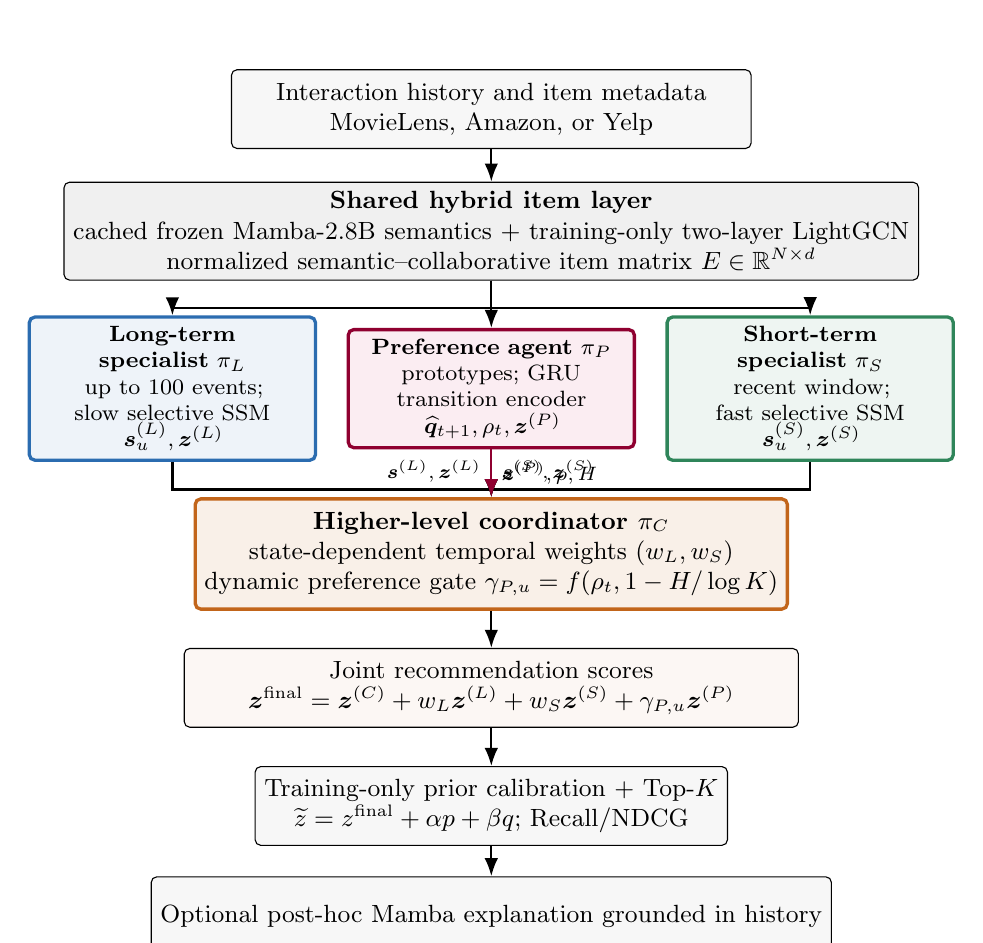
\begin{tikzpicture}[
  box/.style={draw,rounded corners=2pt,align=center,minimum height=10mm,
              minimum width=39mm,fill=black!3,font=\small},
  shared/.style={box,minimum width=92mm,fill=black!6},
  agent/.style={box,text width=34mm,minimum width=34mm,minimum height=14mm,
                font=\footnotesize},
  coordinator/.style={box,minimum width=64mm,minimum height=14mm,
                      draw=agentorange,very thick,fill=agentorange!10},
  arrow/.style={-{Latex[length=2.3mm]},thick},
  feedback/.style={-{Latex[length=2.3mm]},thick,dashed,draw=red!70!black}
]
% Shared observation and representation layer.
\node[box,minimum width=66mm] (data) at (0,0)
  {Interaction history and item metadata\\MovieLens, Amazon, or Yelp};
\node[shared] (semantic) at (0,-1.55)
  {\textbf{Shared hybrid item layer}\\
   cached frozen Mamba-2.8B semantics + training-only two-layer LightGCN\\
   normalized semantic--collaborative item matrix $E\in\R^{N\times d}$};

% Parallel specialist level.
\node[agent,draw=agentblue,very thick,fill=agentblue!8] (long) at (-4.05,-3.55)
  {\textbf{Long-term specialist $\pi_L$}\\
   up to 100 events; slow selective SSM\\
   $\bm s_u^{(L)},\bm z^{(L)}$};
\node[agent,draw=purple!75!black,very thick,fill=purple!7] (pref) at (0,-3.55)
  {\textbf{Preference agent $\pi_P$}\\
   prototypes; GRU transition encoder\\
   $\widehat{\bm q}_{t+1},\rho_t,\bm z^{(P)}$};
\node[agent,draw=agentgreen,very thick,fill=agentgreen!8] (short) at (4.05,-3.55)
  {\textbf{Short-term specialist $\pi_S$}\\
   recent window; fast selective SSM\\
   $\bm s_u^{(S)},\bm z^{(S)}$};

% Higher-level coordination and the deployed action.
\node[coordinator] (coord) at (0,-5.65)
  {\textbf{Higher-level coordinator $\pi_C$}\\
   state-dependent temporal weights $(w_L,w_S)$\\
   dynamic preference gate $\gamma_{P,u}=f(\rho_t,1-H/\log K)$};
\node[box,minimum width=78mm,fill=agentorange!5] (rank) at (0,-7.35)
  {Joint recommendation scores\\
   $\bm z^{\mathrm{final}}=\bm z^{(C)}+w_L\bm z^{(L)}+w_S\bm z^{(S)}
   +\gamma_{P,u}\bm z^{(P)}$};
\node[box,minimum width=55mm] (catalog) at (0,-8.85)
  {Training-only prior calibration + Top-$K$\\
   $\widetilde z=z^{\mathrm{final}}+\alpha p+\beta q$; Recall/NDCG};
\node[box,minimum width=55mm] (reason) at (0,-10.25)
  {Optional post-hoc Mamba explanation grounded in history};

% Inference path.
\draw[arrow] (data)--(semantic);
\draw[arrow] (semantic.south) -- ++(0,-0.35) -| (long.north);
\draw[arrow] (semantic)--(pref);
\draw[arrow] (semantic.south) -- ++(0,-0.35) -| (short.north);
\draw[arrow] (long.south) -- ++(0,-0.35) -| node[pos=0.72,above left,font=\scriptsize]
  {$\bm s^{(L)},\bm z^{(L)}$} (coord.north);
\draw[arrow] (short.south) -- ++(0,-0.35) -| node[pos=0.72,above right,font=\scriptsize]
  {$\bm s^{(S)},\bm z^{(S)}$} (coord.north);
\draw[arrow,draw=purple!75!black] (pref)--node[right,font=\scriptsize]
  {$\bm z^{(P)},\rho, H$} (coord);
\draw[arrow] (coord)--(rank);
\draw[arrow] (rank)--(catalog);
\draw[arrow] (catalog)--(reason);
\end{tikzpicture}}
\caption{Hierarchical cooperative multi-agent Mamba ranking architecture.
Solid arrows show the inference path.}
\label{fig:pipeline}
\end{figure}

The hierarchy assigns complementary responsibilities rather than making the
rankers vote independently. The two temporal specialists extract preferences at
different time scales, and the higher-level coordinator decides their
state-dependent contribution to one deployed ranking. During joint training,
the coordinator and all specialists receive listwise ranking gradients; during
inference, only the solid forward path is executed. Each colored agent box owns
its own LoRA route; no adapter parameters are shared across agent routes.

\subsection{Data and Chronological Splitting}

Every record becomes $(u,i,\tau,t_i)$: user, item, timestamp, and item text. IDs become contiguous integers. Users need at least five positive events by default. MovieLens and Yelp use rating at least four.

\begin{longtable}{p{0.24\textwidth}p{0.27\textwidth}p{0.41\textwidth}}
\caption{Dataset interfaces and item text.}\label{tab:data}\\
\toprule
Argument & Interactions & Item text\\
\midrule
\endfirsthead
\toprule
Argument & Interactions & Item text\\
\midrule
\endhead
movielens & ratings & title and genres\\
amazon-\textless category\textgreater & Amazon Reviews 2023 & title, subtitle, main category, features, description\\
amazon:\textless exact-config\textgreater & exact HF config & review/meta join by \texttt{parent\_asin}\\
yelp19, yelp23 & local Yelp JSON/table & name, categories, location, attributes\\
synthetic & deterministic events & short names for tests\\
\bottomrule
\end{longtable}

Yelp is license-gated and requires a local path. Leave-two-out splitting is
\begin{align}
  \mathcal H_u^{\mathrm{train}}&=(i_1,\ldots,i_{T_u-2}),\\
  i_u^{\mathrm{valid}}&=i_{T_u-1},\\
  i_u^{\mathrm{test}}&=i_{T_u}.
\end{align}
Training prefixes produce $\big((i_1,\ldots,i_k),i_{k+1}\big)$. Reservoir sampling caps transitions at \texttt{MAX\_TRANSITIONS}.

\subsection{Cached Mamba Semantics}

The frozen \texttt{state-spaces/mamba-2.8b-hf} backbone encodes metadata after
the prefix \texttt{Preference-aware product representation:}. The Amazon suite
caps the prompted input at 32 tokens. Prompt tokens condition the causal hidden
states but are excluded from content mean pooling:
\begin{equation}
  \bm e_i^{\mathrm{text}}
  =
  \operatorname{MeanPool}
  \left(\operatorname{Mamba}_{\mathrm{frozen}}(t_i)\right)
  \in\R^{d_m}.
\end{equation}
The prompt, item texts, dataset name, catalog size, and token cap determine the
cache identity, preventing reuse of incompatible vectors. A shared bridge gives
\begin{equation}
  \bm e_i=\operatorname{norm}(W_p\bm e_i^{\mathrm{text}}),
  \qquad W_p\in\R^{d\times d_m},\quad d=128.
\end{equation}

\subsection{Training-Only LightGCN Fusion}

The current implementation enables a two-layer LightGCN branch by default
\cite{LIGHTGCN}. It constructs an undirected bipartite graph only from unique
user--item pairs in \texttt{train\_by\_user}; validation and test edges are
excluded. Let $A$ be its adjacency matrix, $D$ its degree matrix, and
$X^{(0)}\in\R^{(|\mathcal U|+|\mathcal I|)\times d}$ trainable node embeddings.
The code performs symmetric normalized propagation without feature transforms
or nonlinearities:
\begin{align}
  X^{(\ell+1)} &= D^{-1/2}AD^{-1/2}X^{(\ell)},\qquad \ell\in\{0,1\},\\
  \bar X &= \frac{1}{3}\sum_{\ell=0}^{2}X^{(\ell)}.
\end{align}
Writing $\bm e_i^{\mathrm{gcn}}$ for item $i$'s row of $\bar X$, the actual
vector consumed by both specialists and by catalog scoring is
\begin{equation}
  \bm e_i=\operatorname{norm}\!\left(
    \operatorname{norm}(W_p\bm e_i^{\mathrm{text}})+
    \operatorname{norm}(\bm e_i^{\mathrm{gcn}})
  \right).
\end{equation}
Thus the graph is a shared collaborative item encoder, not a fifth agent. It is
optimized with the item projection during specialist warm-up and
joint training, frozen during coordinator warm-up, and recomputed once per
batch for reuse by histories and candidates. The optional
\texttt{--graph-device} places graph parameters and edges on a second GPU;
\texttt{--no-use-graph-embeddings} provides the semantic-only ablation.

\subsection{Agent-Specific LoRA}

For input $\bm x$, agent $j$ owns
\begin{equation}
  \operatorname{LoRA}_j(\bm x)
  =
  \frac{\alpha}{r}B_jA_j\operatorname{Dropout}(\bm x).
\end{equation}
The generic single-dataset launcher defaults to $r=8$ and $\alpha=16$, while
the ver4 Amazon multi-LoRA suite used in this report sets $r=16$ and
$\alpha=32$; both use dropout $0.05$. $A_j$ uses Kaiming initialization and
$B_j$ starts at zero. The complete routing table is shown in
Table~\ref{tab:lora-routing}.

\begin{table}[H]
\centering
\caption{Disjoint LoRA routes in the ver4 multi-LoRA system.}
\label{tab:lora-routing}
\begin{tabular}{lll}
\toprule
Agent & LoRA residuals & Count\\
\midrule
Long-term & candidate, delta, gate, output & 4\\
Short-term & candidate, delta, gate, output & 4\\
Preference-transition & GRU-state transition, prototype-mixture state & 2\\
Coordinator & temporal mixture, fused state, score state & 3\\
\midrule
Total & disjoint automatically routed adapters & 13\\
\bottomrule
\end{tabular}
\end{table}

The adapter bank operates only in the compact recommender. Cached Mamba-2.8B
features are immutable inputs, while the shared projection, LightGCN embeddings,
preference prototypes, GRU and task heads are ordinary trainable recommender
parameters. Thus ``multi-LoRA'' denotes agent-specific low-rank residual routes;
it does not imply adaptation of the Mamba-2.8B backbone.

\subsection{Selective-State Specialists}

For $j\in\{L,S\}$:
\begin{align}
  \bm\delta_t^{(j)}
  &=
  \operatorname{softplus}
  \left(\bm b_\delta^{(j)}+\operatorname{LoRA}^{(j)}_\delta(\bm x_t)\right),\\
  \bm a_t^{(j)}&=\exp(-\bm\delta_t^{(j)}),\\
  \widetilde{\bm h}_t^{(j)}
  &=
  \tanh\left(\bm x_t+\operatorname{LoRA}^{(j)}_{\mathrm{candidate}}(\bm x_t)\right),\\
  \bm h_t^{(j)}
  &=
  \bm a_t^{(j)}\odot\bm h_{t-1}^{(j)}
  +(1-\bm a_t^{(j)})\odot\widetilde{\bm h}_t^{(j)},\\
  \bm g_t^{(j)}
  &=
  \sigmoid\left(\operatorname{LoRA}^{(j)}_{\mathrm{gate}}(\bm x_t)\right),\\
  \bm o_t^{(j)}
  &=
  \bm g_t^{(j)}\odot\bm h_t^{(j)}
  +(1-\bm g_t^{(j)})\odot\bm x_t.
\end{align}
Small $\bm\delta_t$ preserves history; large values adopt the current item. Long sees up to 100 events at initial time scale $0.08$; short sees 10 at $0.5$. Logits are
\begin{equation}
  z_i^{(j)}=\exp(\tau_j)\langle\bm s_u^{(j)},\bm e_i\rangle.
\end{equation}

\subsection{Preference Prototype Discovery and Transition Prediction}
\label{sec:preference-agent}

The preference agent does not require manually labeled preference categories.
It learns $K$ prototype vectors
$P=[\bm p_1;\ldots;\bm p_K]\in\R^{K\times d}$ shared by every user in one
dataset. For normalized item vector $\bm e_t$, its soft pseudo-preference is
\begin{equation}
  \bm q_t
  =
  \softmax\!\left(
    \frac{\operatorname{norm}(\bm e_t)
    \operatorname{norm}(P)^\top}{T_p}
  \right),
  \qquad \bm q_t\in\Delta^{K-1},
\end{equation}
where $T_p=0.2$ by default. These assignments are latent pseudo-preferences,
not human-authored genres or categories.

A GRU reads $(\bm q_1,\ldots,\bm q_t)$. If $\bm h_t^G$ is the last valid GRU
state, an agent-specific LoRA residual produces
\begin{equation}
  \bm h_t^{(P)}
  =\operatorname{LayerNorm}
    \left(\bm h_t^G+\operatorname{LoRA}_{\mathrm{transition}}(\bm h_t^G)\right).
\end{equation}
The LoRA residual begins as an exact no-op because its second matrix is
zero-initialized. The current and predicted-next distributions and the
transition probability are
\begin{align}
  \bm q_t^{\mathrm{current}} &= \bm q_t,\\
  \widehat{\bm q}_{t+1}
    &=\softmax(W_n\bm h_t^{(P)}+\bm b_n),\\
  \ell_t^{\mathrm{change}}
    &=W_c[\bm h_t^{(P)};\bm q_t]+b_c,\\
  \rho_t&=\sigmoid(\ell_t^{\mathrm{change}}).
\end{align}
The next-preference state and candidate logits are
\begin{align}
  \bm v_t&=\widehat{\bm q}_{t+1}\operatorname{norm}(P),\\
  \bm s_u^{(P)}
    &=\operatorname{norm}\!\left(\bm v_t+
      \operatorname{LoRA}_{\mathrm{state}}(\bm v_t)\right),\\
  z_i^{(P)}&=\exp(\tau_P)\langle\bm s_u^{(P)},\bm e_i\rangle.
\end{align}
The state adapter also begins as a no-op. The raw change logit is used for
AMP-safe binary cross entropy with logits; $\rho_t$ is used for analysis and
for the coordinator's context-dependent preference gate.

\begin{figure}[H]
\centering
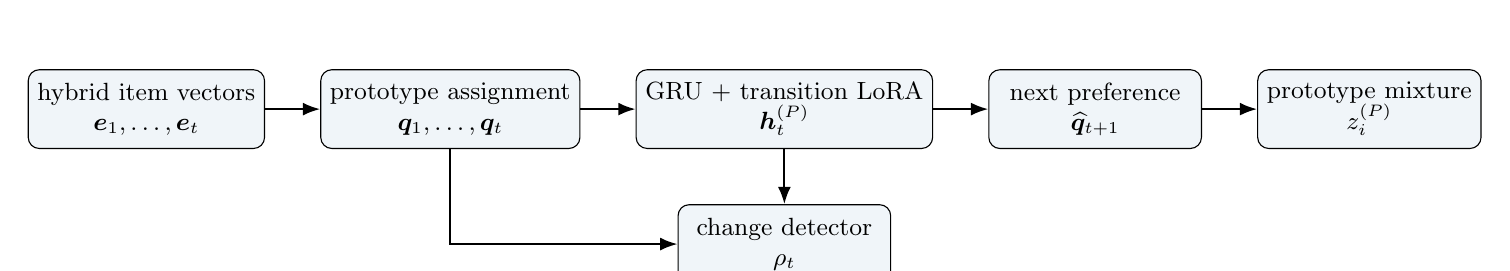
\begin{tikzpicture}[
  pbox/.style={draw,rounded corners,align=center,minimum height=10mm,
               minimum width=27mm,fill=agentblue!7,font=\small},
  parr/.style={-{Latex[length=2.2mm]},thick}
]
\node[pbox] (items) {hybrid item vectors\\$\bm e_1,\ldots,\bm e_t$};
\node[pbox,right=7mm of items] (assign) {prototype assignment\\$\bm q_1,\ldots,\bm q_t$};
\node[pbox,right=7mm of assign] (gru) {GRU + transition LoRA\\$\bm h_t^{(P)}$};
\node[pbox,right=7mm of gru] (next) {next preference\\$\widehat{\bm q}_{t+1}$};
\node[pbox,below=7mm of gru] (change) {change detector\\$\rho_t$};
\node[pbox,right=7mm of next] (score) {prototype mixture\\$z_i^{(P)}$};
\draw[parr] (items)--(assign);
\draw[parr] (assign)--(gru);
\draw[parr] (gru)--(next);
\draw[parr] (gru)--(change);
\draw[parr] (assign.south) |- (change.west);
\draw[parr] (next)--(score);
\end{tikzpicture}
\caption{Preference-transition branch in ver4. Soft assignments expose a
latent preference trajectory; the branch predicts both the next distribution
and the probability of a transition before contributing candidate scores.}
\label{fig:preference-transition}
\end{figure}

\subsection{Preference Training Objectives}

The target item's detached assignment $\bm q^+$ supervises the next
distribution:
\begin{equation}
  \mathcal L_{\mathrm{next}}
  =D_{\mathrm{KL}}(\bm q^+\,\|\,\widehat{\bm q}_{t+1}).
\end{equation}
Transition strength is a soft target derived from Jensen--Shannon divergence:
\begin{align}
  \bm m&=\tfrac12(\bm q_t^{\mathrm{current}}+\bm q^+),\\
  y_t^{\mathrm{change}}
  &=\frac{
    \tfrac12D_{\mathrm{KL}}(\bm q_t^{\mathrm{current}}\|\bm m)
    +\tfrac12D_{\mathrm{KL}}(\bm q^+\|\bm m)}
    {\log 2},\\
  \mathcal L_{\mathrm{change}}
  &=\operatorname{BCEWithLogits}
    (\ell_t^{\mathrm{change}},y_t^{\mathrm{change}}).
\end{align}
If $\bar{\bm q}=B^{-1}\sum_b\bm q_b^+$, two anti-collapse terms are
\begin{align}
  \mathcal L_{\mathrm{balance}}
    &=D_{\mathrm{KL}}(\bar{\bm q}\,\|\,\operatorname{Uniform}(K)),\\
  \mathcal L_{\mathrm{separate}}
    &=\frac1{K^2}\|
      \operatorname{norm}(P)\operatorname{norm}(P)^\top-I
    \|_F^2.
\end{align}
The default auxiliary objective is
\begin{equation}
  \mathcal L_P
  =0.2\mathcal L_{\mathrm{next}}
  +0.1\mathcal L_{\mathrm{change}}
  +0.01\mathcal L_{\mathrm{balance}}
  +0.01\mathcal L_{\mathrm{separate}}.
\end{equation}

\subsection{Coordinator and Final Ranking}

\begin{align}
  \bm q_u&=[\bm s_u^{(L)};\bm s_u^{(S)}],\\
  [w_L,w_S]&=\softmax(\operatorname{LoRA}_{\mathrm{mix}}(\bm q_u)),\\
  \bm s_u^{(C)}
  &=
  \operatorname{norm}\left(
  w_L\bm s_u^{(L)}+w_S\bm s_u^{(S)}
  +\operatorname{LoRA}_{\mathrm{state}}(\bm q_u)\right),\\
  c_t^P&=1-H(\widehat{\bm q}_{t+1})/\log K,\\
  \gamma_{P,u}&=\sigmoid(g_P+f_g[\rho_t;c_t^P]),\\
  z_i^{\mathrm{final}}
  &=z_i^{(C)}+w_Lz_i^{(L)}+w_Sz_i^{(S)}
    +\gamma_{P,u}z_i^{(P)}.
\end{align}
The base scalar $g_P$ is initialized so that $\gamma_{P,u}=0.2$, and $f_g$
starts at zero. Thus the dynamic gate initially reproduces the previous global
weight, then learns user-dependent calibration from transition probability and
next-preference confidence while coordinator warm-up freezes the encoder.

\subsection{Training-Only Catalog Calibration}

The neural coordinator can be augmented by two deterministic catalog priors.
They are estimated strictly from $\mathcal H_u^{\mathrm{train}}$ and therefore
introduce no validation or test interactions into the feature construction.
Let $c_i$ be the number of occurrences of item $i$ in all training histories.
The standardized log-popularity feature is
\begin{equation}
  p_i=
  \frac{\log(1+c_i)-\mu_p}{\max(\sigma_p,10^{-6})}.
\end{equation}
For adjacent training events, let $n_{a,b}$ count transitions from item $a$ to
item $b$ and define
\begin{equation}
  q_{a,b}=\log(1+n_{a,b}).
\end{equation}
If $\ell_u$ is the last observed item in the inference history, the deployed
full-catalog score is
\begin{equation}
  \widetilde z_{u,i}
  =
  z_{u,i}^{\mathrm{final}}
  +\alpha p_i
  +\beta q_{\ell_u,i},
  \qquad q_{\ell_u,i}=0\ \text{for unseen transitions}.
\end{equation}
Seen non-target items are masked after calibration. The coefficients $\alpha$
and $\beta$ are selected using validation ranking only; the held-out test set
is evaluated once after the choice is fixed. A negative $\alpha$ suppresses
over-popular items, while a positive $\beta$ reinforces locally plausible
next-item transitions. This calibration is not an agent and does not update
model weights. Both coefficients default to zero, so existing runs retain the
original neural ranking exactly.

\section{Training Strategy}

\subsection{Training Targets and Hard Negatives}

For every training prefix ending at $t$, up to $H=3$ future items from the
training sequence receive exponentially decayed weights:
\begin{equation}
  \omega_h=\frac{\eta^{h-1}}{\sum_{r=1}^{H_u}\eta^{r-1}},
  \qquad \eta=0.5,\quad h\leq H_u\leq H.
\end{equation}
Validation and test targets are never used to construct these labels. A random
pool four times larger than the required negative set is scored by the current
coordinator. Items occurring in that user's training history are masked, and
the highest-scoring remaining items become model-aware hard negatives. For
agent $j$, the soft listwise loss is
\begin{equation}
  \mathcal L_{\mathrm{rank}}^{(j)}
  =-\sum_{h=1}^{H_u}\omega_h
    \log\softmax(\bm z^{(j)})_{i_{t+h}}.
\end{equation}
The bounded transition set is regenerated with a new deterministic seed every
epoch, so large datasets expose different prefixes without increasing one
epoch's memory budget.

\subsection{Stage 1: Specialist Warm-Up}

The coordinator is frozen:
\begin{equation}
  \mathcal L_{\mathrm{specialist}}
  =
  \mathcal L_{\mathrm{rank}}^{(L)}
  +\mathcal L_{\mathrm{rank}}^{(S)}
  +\mathcal L_{\mathrm{rank}}^{(P)}
  +\mathcal L_P.
\end{equation}

\subsection{Stage 2: Coordinator Warm-Up}

Specialists and projection are frozen:
\begin{equation}
  \mathcal L_{\mathrm{coord}}
  =
  \mathcal L_{\mathrm{rank}}^{(C)}.
\end{equation}

\subsection{Stage 3: Joint Ranking and Preference Alignment}

The preference state is aligned with immediate target item vectors using an
in-batch multi-positive contrastive objective. Samples sharing the same target
are all treated as positives rather than false negatives:
\begin{align}
  \mathcal P_b&=\{r:i_r^+=i_b^+\},\\
  \mathcal L_{\mathrm{contrast}}
  &=
  -\frac1B\sum_b\log
  \frac{\sum_{r\in\mathcal P_b}
    \exp(\operatorname{sim}(\bm s_b^{(P)},\bm e_r^+)/\tau)}
  {\sum_r\exp(\operatorname{sim}(\bm s_b^{(P)},\bm e_r^+)/\tau)},\\
  \mathcal L_{\mathrm{joint}}
  &=
  \frac14\sum_{j\in\{L,S,P,C\}}\mathcal L_{\mathrm{rank}}^{(j)}
  +\mathcal L_P+0.05\mathcal L_{\mathrm{contrast}}.
\end{align}
The previous cosine-squared long/short specialization penalty is removed:
different history windows and decay time scales already provide structural
specialization, while forced orthogonality can discard preference information
shared across temporal scales.

\subsection{Gradients and Optimization}

Coordinator ranking gradients flow through fusion into both specialist paths,
and every specialist receives its own listwise ranking loss.

\begin{table}[H]
\centering
\caption{Optimization used by the ver4 Amazon multi-LoRA suite.}
\begin{tabular}{lccl}
\toprule
Stage & Epochs & Learning rate & Trainable components\\
\midrule
Specialists & 4 & $1\times10^{-4}$ & long, short, preference, projection, LightGCN\\
Coordinator & 4 & $1\times10^{-4}$ & coordinator and preference score gate\\
Joint ranking & 10 & $5\times10^{-5}$ & all recommender components\\
\bottomrule
\end{tabular}
\end{table}
AdamW uses weight decay $10^{-5}$. CUDA uses FP16 autocast, GradScaler, and gradient clipping at 1.0. The Amazon suite uses batch size 128, evaluation batch size 64, dataset-specific candidate counts and validation intervals, and caps the effective interval at one epoch so every epoch is validated. A \texttt{ReduceLROnPlateau} scheduler halves the coordinator or joint learning rate after two non-improving checks, and joint training stops after six non-improving checks. Because the Amazon launcher sets \texttt{SAVE\_MODEL\_WEIGHTS=0}, the best validation state is retained in memory rather than written as a checkpoint; final metrics are computed only after restoring that state.

\section{Full-Catalog Evaluation and Throughput}

Evaluation projects the complete catalog once even though the reported Amazon
runs train with bounded hard-negative slates:
\begin{equation}
  E=\operatorname{HybridProject}(E_{\mathrm{text}},E_{\mathrm{gcn}})
  \in\R^{N\times d},
  \qquad Z^{(j)}=S^{(j)}E^\top\in\R^{B\times N}.
\end{equation}
Each agent applies its learned temperature, and the coordinator combines
$Z^{(L)}$, $Z^{(S)}$, $Z^{(P)}$, and its own adapted-state score to obtain
$Z^{\mathrm{final}}$. Matrix multiplication avoids a $B\times N\times d$
expansion. Popularity and transition vectors are then added by broadcasting
and sparse row updates to obtain $\widetilde Z$; they do not require another
model forward pass. Seen non-target items receive $-\infty$.

\begin{align}
  \operatorname{rank}_u
  &=\sum_{i=1}^N\mathbb{I}[\widetilde z_{u,i}\geq
    \widetilde z_{u,i^+}],\\
  \operatorname{Recall@K}
  &=\frac1{|\mathcal U|}\sum_u\mathbb{I}[\operatorname{rank}_u\leq K],\\
  \operatorname{NDCG@K}
  &=\frac1{|\mathcal U|}\sum_u
  \frac{\mathbb{I}[\operatorname{rank}_u\leq K]}
       {\log_2(\operatorname{rank}_u+1)}.
\end{align}
The code reports $K=5,10$, users/s, and scores/s.

Throughput comes from cached Mamba vectors, shared semantics, linear
selective recurrences, a GRU over 64-dimensional preference assignments, capped
history, bounded listwise candidate sets with model-aware hard negatives, FP16,
GEMM ranking, sparse prior updates, and delayed generator loading.

\section{Recommendation Explanation}

For sampled test users, Top-1, ten recent item texts, and coordinator weights form:
\begin{lstlisting}[language={}]
Explain this recommendation in one concise sentence using only the supplied history.
Long-term agent weight=<wL>; short-term agent weight=<wS>.
History: <recent item texts>.
Recommended item: <recommended item text>. Reason:
\end{lstlisting}
When enabled, Mamba greedily generates at most 40 tokens after ranking. The explanation is grounded but post-hoc; it is not a causal proof and does not affect training or ranking. The Amazon suite used in this report disables reason generation.

\section{Experimental Design}

Required ablations include removal of each of the four agents, identical
versus 100/10 windows, fixed versus learned fusion, random versus model-hard
negatives, one-step versus future soft labels, fixed versus per-epoch prefix
sampling, disjoint versus shared LoRA routes, and alternative LoRA ranks.
Catalog calibration must be ablated as neural-only, popularity-only,
transition-only, and combined scoring, with $\alpha$ and $\beta$ selected on
validation for every dataset. Semantic features should compare Mamba vectors,
random vectors, and ID embeddings. Sequence baselines should include GRU and
Transformer under matched capacity. Random negatives should be compared with
hard negatives.

Beyond Recall/NDCG, useful measures include coverage, novelty, diversity,
results by history length, coordinator-weight distribution, specialist-state
cosine similarity, transitions/s, users/s, scores/s, peak GPU memory, and
explanation latency. Because the priors can change exposure concentration,
coverage and popularity-stratified Recall should accompany aggregate Recall.

\subsection{Completed ver4 Multi-LoRA Result}

Table~\ref{tab:ver4-current} reports the completed multi-LoRA run present in
the version-local output directory at writing time. It uses Amazon Reviews 2023
All Beauty with 1,620 users, 6,982 items, and 11,744 training interactions,
chronological leave-two-out splitting, one held-out item per user, and
full-catalog evaluation. Consequently, Recall and Hit Ratio are identical.
The run uses all 13 LoRA adapters with $r=16$, $\alpha=32$, and dropout $0.05$;
four specialist-stage, four coordinator-stage, and ten joint-stage epochs; 64 training candidates;
and validation-selected catalog coefficients $\alpha_p=-0.25$ and $\beta=4.0$.

\begin{table}[H]
\centering
\caption{Completed ver4 Preference-Transition Multi-LoRA result.}
\label{tab:ver4-current}
\footnotesize
\begin{tabular}{@{}llrrrrrr@{}}
\toprule
Split & Run & $R@5$ & $R@10$ & $H@5$ & $H@10$ & $N@5$ & $N@10$\\
\midrule
Validation & 20260830\_011259 & .09012 & .10123 & .09012 & .10123 & .08258 & .08610\\
Test & 20260830\_011259 & .11358 & .11914 & .11358 & .11914 & .10254 & .10431\\
\bottomrule
\end{tabular}
\end{table}

This is an engineering measurement, not a paper-to-paper victory claim.
Published results may use different Amazon releases, category definitions,
core filters, and candidate protocols. A controlled comparison requires
rerunning baselines through the same loader and evaluator.

The active Beauty and Personal Care job is not included because its log does
not yet contain final validation and test artifacts. Results from predecessor
versions are deliberately excluded from the ver4 result table.

\section{Implementation and Reproducibility}

\begin{table}[H]
\centering
\caption{Independent implementation files.}
\begin{tabularx}{\textwidth}{>{\ttfamily}p{0.34\textwidth}X}
\toprule
File & Responsibility\\
\midrule
run\_mamba\_rl.sh & single-dataset multi-LoRA launcher\\
run\_amazons\_full\_rl.sh & Amazon multi-LoRA suite and subset settings\\
src/data\_mamba\_rl.py & dataset adapters\\
src/model\_mamba\_rl.py & four agents and disjoint LoRA routing\\
src/train\_mamba\_rl.py & training, evaluation, explanations\\
tests/test\_mamba\_rl.py & tests\\
outputs\_mamba\_rl/ & artifacts\\
\bottomrule
\end{tabularx}
\end{table}

\begin{lstlisting}[language=bash]
bash run_mamba_rl.sh movielens-1m 0
bash run_mamba_rl.sh movielens-20m 0
bash run_mamba_rl.sh amazon-all-beauty 0
bash run_mamba_rl.sh amazon-movies-and-tv 0
bash run_mamba_rl.sh yelp19 0 /data/yelp-2019
bash run_mamba_rl.sh yelp23 0 /data/yelp-2023
\end{lstlisting}

Environment variables include \texttt{CACHE\_DIR},
\texttt{BATCH\_SIZE}, \texttt{EVAL\_BATCH\_SIZE},
\texttt{SPECIALIST\_EPOCHS}, \texttt{COORDINATOR\_EPOCHS},
\texttt{JOINT\_EPOCHS}, \texttt{VALIDATE\_EVERY\_STEPS},
\texttt{MONITOR\_METRIC}, \texttt{EARLY\_STOPPING\_PATIENCE},
\texttt{LR\_PATIENCE}, \texttt{MAX\_TRANSITIONS}, \texttt{SEED},
\texttt{POPULARITY\_ALPHA}, \texttt{TRANSITION\_BETA},
\texttt{USE\_GRAPH\_EMBEDDINGS}, \texttt{GRAPH\_DEVICE},
\texttt{TARGET\_RECALL\_AT\_10}, \texttt{EXPERIMENT\_NOTE},
\texttt{LORA\_RANK}, \texttt{LORA\_ALPHA}, \texttt{LORA\_DROPOUT},
\texttt{PREFERENCE\_COUNT}, \texttt{PREFERENCE\_HIDDEN},
\texttt{PREFERENCE\_TEMPERATURE}, \texttt{PREFERENCE\_SCORE\_WEIGHT},
\texttt{PREFERENCE\_COEF}, \texttt{PREFERENCE\_TRANSITION\_COEF},
\texttt{PREFERENCE\_BALANCE\_COEF}, and
\texttt{PREFERENCE\_SEPARATION\_COEF}. The version-local Amazon suite is
\begin{lstlisting}[language=bash]
cd /workspace/P78123011/MediaTek_2026_project/ver4
bash run_amazons_full_rl.sh
\end{lstlisting}
A CPU smoke test is
\begin{lstlisting}[language=bash]
python -m src.train_mamba_rl \
  --dataset synthetic --device cpu --skip-mamba \
  --no-generate-reasons --max-transitions 32 --batch-size 8
\end{lstlisting}

The Amazon suite deliberately disables weight persistence. Its outputs are
\texttt{train\_<run-id>.log}, subset score JSON, \texttt{loss.png},
\texttt{metrics.json}, \texttt{recommendations.json}, and
\texttt{preference\_analysis.json} under
\texttt{outputs\_mamba\_rl/amazons\_lora/<subset>/rl\_<timestamp>/}. Every log begins with
\texttt{EXPERIMENT\_NOTE} and the complete serialized
\texttt{EXPERIMENT\_CONFIG}; calibrated runs additionally record
\texttt{ADAPTATION\_MODE mode=multi\_lora}, \texttt{ADAPTER\_ROUTES},
\texttt{CATALOG\_PRIORS}, vector provenance, an optional resumed checkpoint,
\texttt{VALID\_BEST}, \texttt{TEST\_FINAL}, and
\texttt{TARGET\_RESULT}. Legacy training paths do not import this pipeline.

\section{Limitations}

\begin{enumerate}
  \item Static logs contain no action-dependent user response, so the current
  multi-LoRA system is an offline sequential ranker rather than a complete
  long-horizon MDP.
  \item Random negatives may be unexposed; no propensity correction is used.
  \item Model-mined negatives reduce but do not eliminate the mismatch between
  sampled training and full-catalog evaluation.
  \item Popularity and first-order transition counts are simple, dataset-dependent priors and may not transfer across domains or temporal shifts.
  \item Calibrated gains must be separated from gains in the learned neural ranker; the priors are deterministic post-training score corrections.
  \item Explanations are post-hoc and not optimized for faithfulness.
  \item Latent preference IDs have no guaranteed human semantic label and may
  permute across independent runs or datasets.
  \item A high predicted transition probability identifies a learned embedding
  shift, not a causal change in a person's underlying taste.
  \item Mamba-2.8B supplies frozen item semantics; the agent-specific LoRA bank
  adapts compact recommendation modules rather than the language-model backbone.
\end{enumerate}

Recall/NDCG gains therefore mean improved offline ranking, not proven long-term satisfaction.

\section{Future Research}

Reward-adaptive memory can use
\begin{equation}
  \bm\delta_t=f_\theta(\bm x_t,r_{t-1},\sigma_{t-1}).
\end{equation}
Offline RL can add propensity weighting or
\begin{equation}
  \mathcal L_{\mathrm{CQL}}
  =
  \log\sum_a\exp Q(s,a)-Q(s,a_{\mathrm{logged}}).
\end{equation}
A simulator can support centralized critics and retention reward. Item selection and reasoning can be jointly optimized with
\begin{equation}
  r=
  \lambda_1r_{\mathrm{rank}}
  +\lambda_2r_{\mathrm{grounding}}
  +\lambda_3r_{\mathrm{consistency}}
  +\lambda_4r_{\mathrm{diversity}}.
\end{equation}

\section{Conclusion}

The pipeline combines Mamba item semantics, linear selective-state modeling,
a GRU preference-transition model, and 13 agent-specific LoRA adapters without
fine-tuning or duplicating the Mamba-2.8B backbone. The frozen backbone
establishes a reusable semantic catalog; long and short agents model different
time scales; the preference agent predicts latent preference transitions; and
the coordinator learns context-dependent fusion. Staged multi-step listwise
training establishes the specialists, calibrates coordination, and jointly
adapts the multi-LoRA recommender. Training-only popularity and transition priors
provide a leakage-controlled calibration layer whose effect remains explicitly
separable from learned model quality. Periodic validation, best-state
restoration, auditable experiment logs, and full-catalog evaluation make ranking
quality and systems cost measurable.

\begin{thebibliography}{99}
\bibitem{LORA} E. Hu, Y. Shen, P. Wallis, et al. LoRA: Low-Rank Adaptation of Large Language Models. \emph{ICLR}, 2022.
\bibitem{MAMBA} A. Gu and T. Dao. Mamba: Linear-Time Sequence Modeling with Selective State Spaces. \emph{COLM}, 2024.
\bibitem{RLSURVEY} M. M. Afsar, T. Crump, and B. Far. Reinforcement Learning Based Recommender Systems: A Survey. \emph{ACM Computing Surveys}, 2022.
\bibitem{DRN} G. Zheng, F. Zhang, Z. Zheng, et al. DRN: A Deep Reinforcement Learning Framework for News Recommendation. \emph{The Web Conference}, 2018.
\bibitem{TOPKREINFORCE} M. Chen, A. Beutel, P. Covington, et al. Top-K Off-Policy Correction for a REINFORCE Recommender System. \emph{WSDM}, 2019.
\bibitem{SLATEQ} E. Ie, V. Jain, J. Wang, et al. Reinforcement Learning for Slate-Based Recommender Systems. \emph{arXiv:1905.12767}, 2019.
\bibitem{UNEXPECTEDRL} A. L. Silva, D. Parra, and R. T. Icarte. On the Unexpected Effectiveness of Reinforcement Learning for Sequential Recommendation. \emph{ICML}, 2024.
\bibitem{MAMBA4REC} C. Liu, J. Lin, J. Wang, et al. Mamba4Rec: Towards Efficient Sequential Recommendation with Selective State Space Models. \emph{arXiv:2403.03900}, 2024.
\bibitem{SIGMA} Z. Liu, Q. Liu, Y. Wang, et al. SIGMA: Selective Gated Mamba for Sequential Recommendation. \emph{AAAI}, 2025.
\bibitem{RESID} Y. Liang, Z. Zhang, Y. Zhu, et al. Rethinking Generative Recommender Tokenizer: Recsys-Native Encoding and Semantic Quantization Beyond LLMs. \emph{arXiv:2602.02338}, 2026.
\bibitem{IDIOMOE} R. Shirkavand, X. Wei, C. Wang, et al. Catalog-Native LLM: Speaking Item-ID Dialect with Less Entanglement for Recommendation. \emph{ICLR}, 2026.
\bibitem{BLAIR} Y. Hou, J. Li, X. Fu, et al. Bridging Language and Items for Retrieval and Recommendation: Benchmarking LLMs as Semantic Encoders. \emph{arXiv:2403.03952v2}, 2026.
\bibitem{MARS} H. Kim, J. Kim, M. Choi, S. Lee, and J. Lee. MARS: Matching Attribute-aware Representations for Text-based Sequential Recommendation. \emph{CIKM}, 2024.
\bibitem{HM2REC} Y. Liu, L. Qi, X. Mao, et al. Hyperbolic-Enhanced Mixture-of-Experts Mamba for Sequential Recommendation. \emph{AAAI}, 2026.
\bibitem{MQSATED} T. Zhu, Y. Shi, Y. Zhang, Y. Wu, F. Mo, and J.-Y. Nie. Collaboration and Transition: Distilling Item Transitions into Multi-Query Self-Attention for Sequential Recommendation. \emph{WSDM}, 2024.
\bibitem{DUOREC} R. Qiu, Z. Huang, H. Yin, and Z. Wang. Contrastive Learning for Representation Degeneration Problem in Sequential Recommendation. \emph{WSDM}, 2022.
\bibitem{FMLPREC} K. Zhou, H. Yu, W. X. Zhao, and J. R. Wen. Filter-Enhanced MLP Is All You Need for Sequential Recommendation. \emph{The Web Conference}, 2022.
\bibitem{JGCF} J. Guo, L. Du, X. Chen, et al. On Manipulating Signals of User--Item Graph: A Jacobi Polynomial-Based Graph Collaborative Filtering. \emph{KDD}, 2023.
\bibitem{FASHIONRETRIEVAL} M. Pandey. Domain-Adaptive and Scalable Dense Retrieval for Content-Based Recommendation. \emph{arXiv:2602.00899}, 2026.
\bibitem{LIGHTGCN} X. He, K. Deng, X. Wang, Y. Li, Y. Zhang, and M. Wang. LightGCN: Simplifying and Powering Graph Convolution Network for Recommendation. \emph{SIGIR}, 2020.
\bibitem{AMIM} Y. Cheng, Y. Fan, Y. Wang, and X. Li. Accurate Multi-Interest Modeling for Sequential Recommendation with Attention and Distillation Capsule Network. \emph{Expert Systems with Applications}, vol. 243, article 122887, 2024.
\bibitem{PAAC} M. Cai, L. Chen, Y. Wang, H. Bai, P. Sun, L. Wu, M. Zhang, and M. Wang. Popularity-Aware Alignment and Contrast for Mitigating Popularity Bias. \emph{KDD}, 2024.
\bibitem{DIFFURECSYS} S. Zolghadr, O. Winther, and P. Jeha. Generative Diffusion Models for Sequential Recommendations. \emph{RecSys 2024 Workshop / arXiv:2410.19429}, 2024.
\bibitem{BSAREC} Y. Shin, J. Choi, H. Wi, and N. Park. An Attentive Inductive Bias for Sequential Recommendation beyond the Self-Attention. \emph{AAAI}, 2024.
\bibitem{BSARECREPRO} J. Hutter, H. C. Bakker, S. Fris, M. Bernardy, and Y. Liu. A Systematic Reproducibility Study of BSARec for Sequential Recommendation. \emph{arXiv:2512.17442}, 2025.
\bibitem{HOLOMAMBA} A. Parthasarathy, A. M. Kirubakaran, V. Punniyamoorthy, et al. Scalable Sequential Recommendation under Latency and Memory Constraints. \emph{arXiv:2601.08360}, 2026.
\end{thebibliography}

\end{document}
